\documentclass[12pt]{article}

% =========================
% Toggle: show only problems, or problems + student solution boxes
% =========================
\newif\ifsolutions
\solutionstrue     % Use this for the student template with solution boxes.
%\solutionsfalse   % Use this for a question sheet only.

% =========================
% Packages
% =========================
\usepackage[a4paper,margin=24mm]{geometry}
\usepackage{amsmath,amssymb,mathtools}
\usepackage{braket}
\usepackage{siunitx}
\usepackage[most]{tcolorbox}
\usepackage{enumitem}
\usepackage{graphicx}
\usepackage{xcolor}
\usepackage[T1]{fontenc}
\usepackage{lmodern}
\usepackage{microtype}
\usepackage{float} % Allows figure to be placed at exact desired location
\usepackage[hidelinks]{hyperref}

\sisetup{inter-unit-product = \ensuremath{{}\cdot{}}}
\renewcommand{\d}{\mathop{}\!\mathrm{d}}
\setlength{\parindent}{0pt}
\setlength{\parskip}{0.55em}
\setlist[enumerate,1]{label=(\alph*),itemsep=0.25em,topsep=0.25em}
\setlist[enumerate,2]{label=(\roman*),itemsep=0.15em,topsep=0.15em}

% =========================
% Boxes
% =========================
\tcbset{
  enhanced,
  breakable,
  boxrule=0.8pt,
  arc=1.5mm,
  left=2mm,right=2mm,top=1.5mm,bottom=1.5mm
}

\newtcolorbox{problembox}[1]{
  colback=gray!8,
  colframe=black,
  fonttitle=\bfseries,
  title={#1}
}

\newtcolorbox{solutionbox}{
  colback=blue!3,
  colframe=blue!60!black,
  title={Solution},
  fonttitle=\bfseries
}

\newtcolorbox{answerbox}{
  colback=yellow!10,
  colframe=orange!70!black,
  title={Final answer},
  fonttitle=\bfseries
}

\newtcolorbox{insightbox}{
  colback=green!5,
  colframe=green!50!black,
  title={Physical insight},
  fonttitle=\bfseries
}

\newcommand{\problemsep}{\vspace{0.8em}}

\newcommand{\placeholderfigure}[2][50mm]{%
\begin{center}
\fbox{\parbox[c][#1][c]{0.82\linewidth}{\centering\small Figure placeholder}}\\[0.3em]
{\footnotesize\emph{Caption: #2}}
\end{center}}

\graphicspath{{figures/}} % If you want to place figures in the folder 'figures' (cleaner)

\setcounter{secnumdepth}{0} % Avoids numbering of the section and subsection while allowing them to appear in the TOC



% ======================================================
% ======================================================
% ================                    ==================
% ================   BEGIN DOCUMENT   ==================
% ================                    ==================
% ======================================================
% ======================================================

\begin{document}

\begin{center}
{\Large\bfseries QT01 -- Foundations of Quantum Mechanics\\[0.2em]
Assessed problem set (PRB) -- Week 4\\[0.3em]
{\normalsize Weight: 30\% of module grade}\\[1em]
Candidate number: 672128
}
\end{center}


% ======================================================
%                  Question 1
% ======================================================
\section{Question 1 (Canvas question 1)}
\begin{problembox}{Question 1 \hfill [8 marks]}
Consider the operator
\[
    \hat{A} = \begin{pmatrix} -3 & 2i \\ -2i & -3 \end{pmatrix}.
\]
Prove that \( \hat{A} \) is Hermitian.
\end{problembox}

% ======================================================
%                  Solution 1
% ======================================================
\ifsolutions
\begin{solutionbox}
\textbf{What is asked.} Show that the matrix $\hat{A}$ is equal to its own adjoint.

\textbf{Principle used.} An operator is Hermitian when it coincides with its adjoint,
\[
    \hat{A}=\hat{A}^{\dagger},
\]
which is the condition an operator must satisfy in order to represent a physical observable. For an operator acting on a finite-dimensional space, that is, for a matrix, the adjoint is obtained by transposing the matrix and complex conjugating each of its entries,
\[
    \hat{A}^{\dagger}=\left(\hat{A}^{\mathsf{T}}\right)^{*}.
\]
The proof therefore consists of carrying out those two operations and comparing the outcome with the original matrix.

\textbf{Step 1: transpose.} Exchanging rows and columns, that is, reflecting the entries about the leading diagonal,
\[
    \hat{A}^{\mathsf{T}}
    =\begin{pmatrix} -3 & 2i \\ -2i & -3 \end{pmatrix}^{\mathsf{T}}
    =\begin{pmatrix} -3 & -2i \\ 2i & -3 \end{pmatrix}.
\]

\textbf{Step 2: complex conjugate.} Now conjugate every entry, that is, replace $i$ by $-i$ wherever it appears:
\[
    \hat{A}^{\dagger}=\left(\hat{A}^{\mathsf{T}}\right)^{*}
    =\begin{pmatrix} -3 & -2i \\ 2i & -3 \end{pmatrix}^{*}
    =\begin{pmatrix} -3 & 2i \\ -2i & -3 \end{pmatrix}.
\]

\textbf{Step 3: compare.} The final matrix is entry by entry identical to $\hat{A}$, so $\hat{A}^{\dagger}=\hat{A}$ and the operator is Hermitian.

Equivalently, in components the condition reads $A_{ij}=A_{ji}^{*}$: both diagonal entries are real, and the off-diagonal entries $2i$ and $-2i$ are complex conjugates of one another, which is exactly what Hermiticity demands of a $2\times 2$ matrix.

\textbf{Check: the eigenvalues must come out real.} A Hermitian operator is guaranteed to have real eigenvalues, so computing them is an independent test of the result above. The characteristic equation is
\[
    \det\left(\hat{A}-\lambda I\right)
    =\begin{vmatrix} -3-\lambda & 2i \\ -2i & -3-\lambda \end{vmatrix}
    =(-3-\lambda)^{2}-(2i)(-2i)=0 .
\]
Since $(2i)(-2i)=-4i^{2}=4$, this reduces to
\[
    (\lambda+3)^{2}=4 \quad\Longrightarrow\quad \lambda+3=\pm 2 ,
\]
so that
\[
    \lambda_{1}=-1, \qquad \lambda_{2}=-5 .
\]
Both are real, as they must be for a Hermitian operator, which independently confirms the result.
\end{solutionbox}

\begin{answerbox}
\[
    \hat{A}^{\dagger}=\left(\hat{A}^{\mathsf{T}}\right)^{*}
    =\begin{pmatrix} -3 & 2i \\ -2i & -3\end{pmatrix}=\hat{A},
\]
so $\hat{A}$ is Hermitian. Its eigenvalues, $\lambda_{1}=-1$ and $\lambda_{2}=-5$, are real, as Hermiticity requires.
\end{answerbox}

\begin{insightbox}
This matrix is a spin operator in disguise. Since
\[
    \hat{A}=-3\,I-2\hat{\sigma}_{y},
    \qquad
    \hat{\sigma}_{y}=\begin{pmatrix} 0 & -i \\ i & 0\end{pmatrix},
\]
and $\hat{\sigma}_{y}$ has eigenvalues $\pm 1$, the eigenvalues of $\hat{A}$ must be $-3\mp 2$, that is $-5$ and $-1$, which reproduces the characteristic-equation result without a determinant. Adding a multiple of the identity shifts every eigenvalue by the same amount but leaves every eigenvector unchanged, so $\hat{A}$ measures the same physical property as $\hat{\sigma}_{y}$, on a shifted and rescaled scale.
\end{insightbox}
\fi

\newpage
% ======================================================
%                  Question 2
% ======================================================
\section{Question 2 (Canvas questions 2--5)}
\begin{problembox}{Question 2 \hfill [37 marks]}
The wave function of a particle moving in one dimension is given by
\[
    \psi(x) = \begin{cases}
        B \exp(\beta x) & \text{for } x<0,\\
        B \exp(-2\beta x) & \text{for } x \ge 0,
    \end{cases}
\]
where \(\beta\) is a real and positive constant.

\begin{enumerate}
    \item What is the probability density for finding the particle along the \(x\)-axis? Sketch the probability density function. \hfill [7 marks]
    \item Calculate the normalisation constant \(B\). \hfill [10 marks]
    \item Calculate the average position of the particle on the \(x\)-axis, as a function of \(\beta\). Mark the average position in your sketch. \hfill [15 marks]
    \item Mark the most likely position of the particle in your sketch. \hfill [5 marks]
\end{enumerate}

\textit{Hint: You can calculate the integrals you need by expressing powers of \(x\) through repeated differentiation with respect to the parameter in the exponential, for example}
\begin{align*}
    \int_a^b x \exp(\gamma x)\,\d x
    &= \frac{\partial}{\partial \gamma} \int_a^b \exp(\gamma x)\,\d x, \\
    \int_a^b x^2 \exp(\gamma x)\,\d x
    &= \frac{\partial^2}{\partial \gamma^2} \int_a^b \exp(\gamma x)\,\d x,
\end{align*}
\textit{and so on.}
\end{problembox}

% ======================================================
%                  Solution 2
% ======================================================
\ifsolutions
\begin{solutionbox}

\textbf{(a) The probability density, and its sketch. \hfill (Canvas Q2)}

\textbf{Principle used.} The wave function itself is not directly measurable. What is measurable is the probability density for finding the particle at position $x$, given by the modulus square of the wave function,
\[
    \rho(x)=|\psi(x)|^{2}=\psi^{*}(x)\psi(x),
\]
so that $\rho(x)\,\d x$ is the probability of finding the particle in the interval between $x$ and $x+\d x$. This is the position-space statement of the Born rule.

\textbf{Applying it.} The exponentials are real for real $x$ and $\beta$, so squaring the modulus only affects the constant $B$, giving $|B|^{2}$. Squaring each branch separately,
\[
    \rho(x)=|\psi(x)|^{2}=
    \begin{cases}
        |B|^{2}\exp(2\beta x), & x<0,\\[0.3em]
        |B|^{2}\exp(-4\beta x), & x\ge 0 .
    \end{cases}
\]
Note that each exponent has doubled, because $\left|e^{\alpha x}\right|^{2}=e^{2\alpha x}$ for real $\alpha$.

\textbf{Features that the sketch must show.} Three properties fix the shape of the curve.

\begin{enumerate}
    \item \emph{It is continuous at the origin and peaks there.} Approaching from either side, $\rho(0^{-})=\rho(0^{+})=|B|^{2}$, so the two branches join. Since $\beta>0$, the left branch $e^{2\beta x}$ rises as $x$ increases towards $0$, and the right branch $e^{-4\beta x}$ falls as $x$ increases away from $0$. The density therefore has its largest value at $x=0$.
    \item \emph{It decays to zero in both directions,} as $e^{2\beta x}\to 0$ when $x\to-\infty$ and $e^{-4\beta x}\to 0$ when $x\to+\infty$. This is what makes the function normalisable, and it is checked explicitly in part (b).
    \item \emph{It is asymmetric.} The characteristic decay length of the density is $1/(2\beta)$ on the left but only $1/(4\beta)$ on the right, these being the distances over which $\rho$ falls by a factor of $e$. The density is therefore spread twice as far to the left of the origin as to the right, and the curve is visibly lopsided.
\end{enumerate}

A fourth feature is worth recording because it is easy to miss. The slopes of the two branches at the origin are
\[
    \left.\frac{\d\rho}{\d x}\right|_{0^{-}}=2\beta|B|^{2},
    \qquad
    \left.\frac{\d\rho}{\d x}\right|_{0^{+}}=-4\beta|B|^{2},
\]
which are not equal. The maximum at $x=0$ is therefore a sharp corner, or cusp, rather than a smooth turning point. This matters in part (d).

The resulting curve is drawn in Fig.~(\ref{fig:psi_proba}), where the normalisation constant found in part (b) has been used to fix the vertical scale, and where the average and most likely positions obtained in parts (c) and (d) are marked.

\begin{figure}[H]
    \centering
    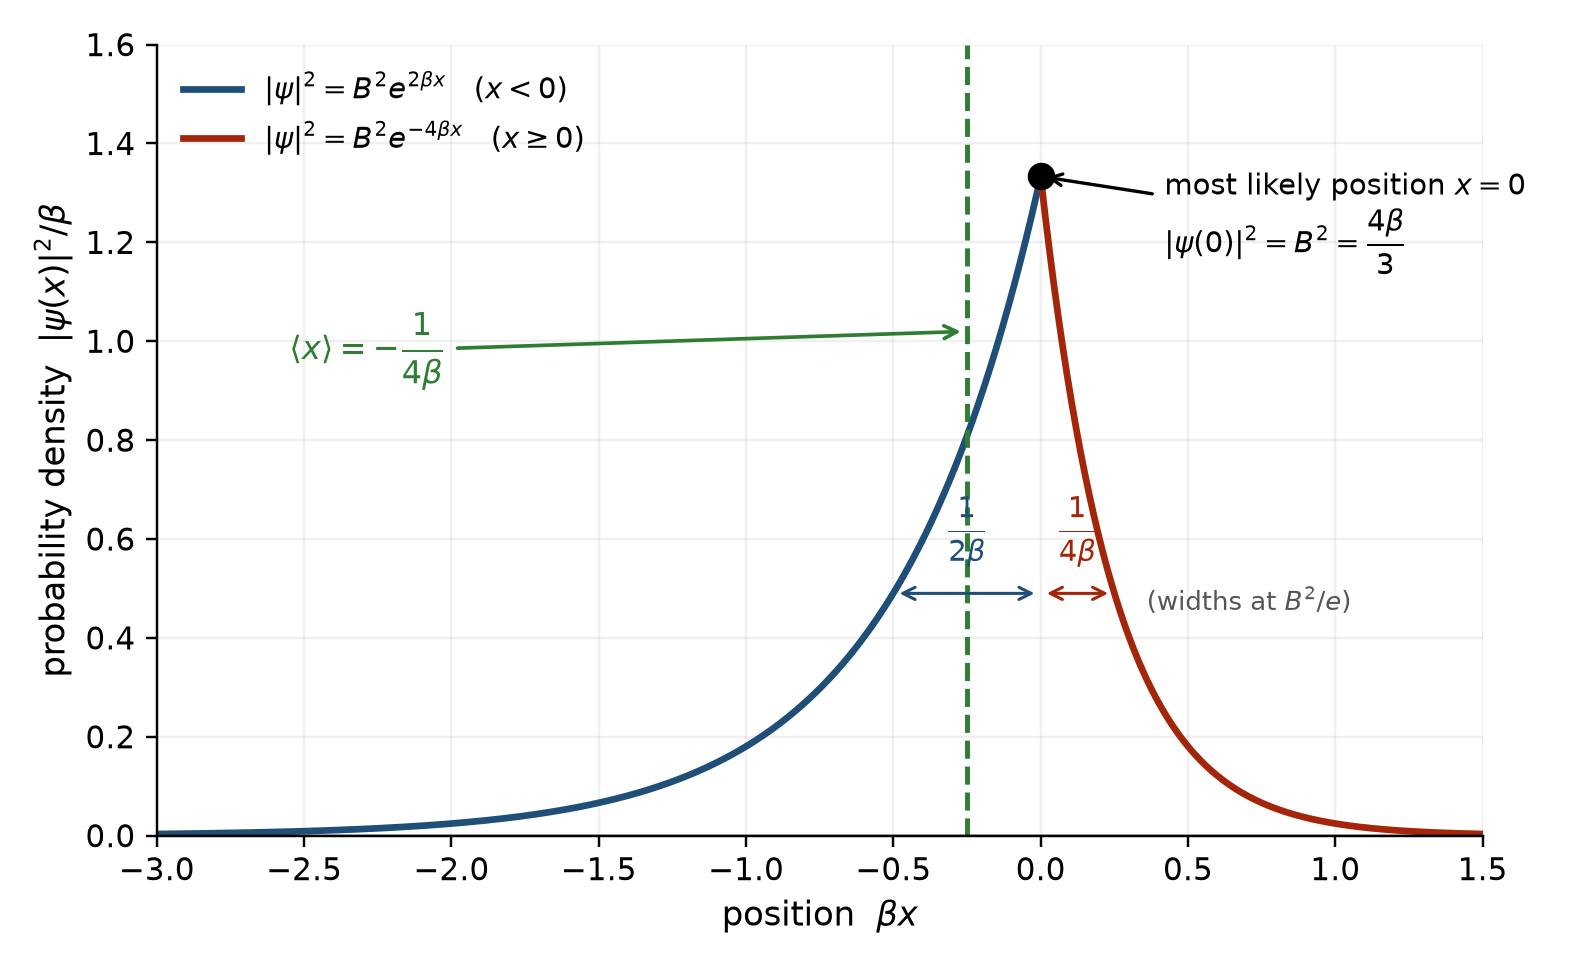
\includegraphics[width=0.92\textwidth]{psi_probability_density.png}
    \caption{The probability density $|\psi(x)|^{2}$, plotted in dimensionless units so that the curve is valid for any $\beta>0$: the horizontal axis is $\beta x$ and the vertical axis is $|\psi(x)|^{2}/\beta$. The density rises as $e^{2\beta x}$ for $x<0$, falls as $e^{-4\beta x}$ for $x\ge 0$, and peaks at the cusp at $x=0$ with the value $B^{2}=4\beta/3$. The horizontal arrows mark the decay lengths $1/(2\beta)$ and $1/(4\beta)$, at which the density has fallen to $B^{2}/e$; the left-hand tail is twice as extended as the right-hand one. The dashed vertical line marks the average position $\langle x\rangle=-1/(4\beta)$, which lies to the left of the peak because of that asymmetry.}
    \label{fig:psi_proba}
\end{figure}

\problemsep
\textbf{(b) The normalisation constant $B$. \hfill (Canvas Q3)}

\textbf{Principle used.} The particle must be found somewhere on the $x$-axis, so the total probability must equal one:
\[
    \int_{-\infty}^{\infty}|\psi(x)|^{2}\,\d x=1 .
\]
This condition determines $|B|$.

\textbf{Splitting the integral.} The wave function is defined by different expressions on either side of the origin, so the integral splits at $x=0$:
\[
    \int_{-\infty}^{\infty}|\psi(x)|^{2}\,\d x
    =|B|^{2}\int_{-\infty}^{0}e^{2\beta x}\,\d x
    +|B|^{2}\int_{0}^{\infty}e^{-4\beta x}\,\d x .
\]

\textbf{The two integrals.} Both are elementary. For the left-hand one, the exponential vanishes at the lower limit because $\beta>0$:
\[
    \int_{-\infty}^{0}e^{2\beta x}\,\d x
    =\left[\frac{e^{2\beta x}}{2\beta}\right]_{-\infty}^{0}
    =\frac{1}{2\beta}-0=\frac{1}{2\beta}.
\]
For the right-hand one, the exponential vanishes at the upper limit:
\[
    \int_{0}^{\infty}e^{-4\beta x}\,\d x
    =\left[-\frac{e^{-4\beta x}}{4\beta}\right]_{0}^{\infty}
    =0-\left(-\frac{1}{4\beta}\right)=\frac{1}{4\beta}.
\]
The right-hand contribution is half the left-hand one, which is the quantitative form of the asymmetry noted in part (a).

\textbf{Solving for $B$.} Adding the two contributions and imposing normalisation,
\[
    |B|^{2}\left(\frac{1}{2\beta}+\frac{1}{4\beta}\right)
    =|B|^{2}\,\frac{2+1}{4\beta}
    =\frac{3|B|^{2}}{4\beta}=1 ,
\]
so that
\[
    |B|^{2}=\frac{4\beta}{3},
    \qquad
    |B|=\sqrt{\frac{4\beta}{3}}=2\sqrt{\frac{\beta}{3}} .
\]
Only the modulus of $B$ is fixed by this condition: multiplying $\psi$ by a phase factor $e^{i\theta}$ leaves $|\psi|^{2}$, and hence every measurable prediction, unchanged. It is conventional to take that free phase to be zero and to quote the real, positive root,
\[
    B=2\sqrt{\frac{\beta}{3}}=\frac{2\sqrt{\beta}}{\sqrt{3}} .
\]

\textbf{Check: dimensions.} The quantity $\beta$ appears in the combination $\beta x$, which must be dimensionless, so $\beta$ has dimensions of inverse length. Then $|B|=\sqrt{4\beta/3}$ has dimensions of (length)$^{-1/2}$, which is exactly right for a one-dimensional wave function, since $|\psi|^{2}\,\d x$ must be a pure number. Using this value, the peak of the density is $\rho(0)=|B|^{2}=4\beta/3$, which is the height marked in Fig.~(\ref{fig:psi_proba}).

\problemsep
\textbf{(c) The average position. \hfill (Canvas Q4)}

\textbf{Principle used.} The average, or expectation, value of an observable in a normalised state is obtained by sandwiching the corresponding operator between the state and its conjugate. For position, whose operator acts simply by multiplication, $\hat{x}\psi(x)=x\psi(x)$, this reads
\[
    \langle \hat{x}\rangle
    =\int_{-\infty}^{\infty}\psi^{*}(x)\,\hat{x}\,\psi(x)\,\d x
    =\int_{-\infty}^{\infty}x\,|\psi(x)|^{2}\,\d x .
\]
This is the familiar mean of a distribution, with $|\psi(x)|^{2}$ playing the role of the probability density. It is legitimate to use this form, rather than dividing by $\braket{\psi|\psi}$, precisely because $B$ has already been chosen in part (b) to make the state normalised.

\textbf{Setting up.} Splitting at the origin as before,
\[
    \langle \hat{x}\rangle
    =|B|^{2}\underbrace{\int_{-\infty}^{0}x\,e^{2\beta x}\,\d x}_{\textstyle I_{-}}
    +|B|^{2}\underbrace{\int_{0}^{\infty}x\,e^{-4\beta x}\,\d x}_{\textstyle I_{+}} .
\]

\textbf{Evaluating the integrals by differentiating with respect to the exponent.} Following the hint, a factor of $x$ in the integrand can be generated by differentiating the corresponding exponential integral with respect to the parameter $\gamma$ in $e^{\gamma x}$, because $\partial e^{\gamma x}/\partial\gamma=x\,e^{\gamma x}$.

For the left-hand integral, define, for $\gamma>0$ so that the integral converges,
\[
    F(\gamma)\equiv\int_{-\infty}^{0}e^{\gamma x}\,\d x
    =\left[\frac{e^{\gamma x}}{\gamma}\right]_{-\infty}^{0}=\frac{1}{\gamma} .
\]
Differentiating both sides with respect to $\gamma$,
\[
    \int_{-\infty}^{0}x\,e^{\gamma x}\,\d x
    =\frac{\partial}{\partial\gamma}\left(\frac{1}{\gamma}\right)
    =-\frac{1}{\gamma^{2}} ,
\]
and setting $\gamma=2\beta$ gives
\[
    I_{-}=-\frac{1}{(2\beta)^{2}}=-\frac{1}{4\beta^{2}} .
\]

For the right-hand integral, define, for $\gamma<0$ so that the integral converges,
\[
    G(\gamma)\equiv\int_{0}^{\infty}e^{\gamma x}\,\d x
    =\left[\frac{e^{\gamma x}}{\gamma}\right]_{0}^{\infty}=-\frac{1}{\gamma} .
\]
Differentiating with respect to $\gamma$,
\[
    \int_{0}^{\infty}x\,e^{\gamma x}\,\d x
    =\frac{\partial}{\partial\gamma}\left(-\frac{1}{\gamma}\right)
    =\frac{1}{\gamma^{2}} ,
\]
and setting $\gamma=-4\beta$ gives
\[
    I_{+}=\frac{1}{(-4\beta)^{2}}=\frac{1}{16\beta^{2}} .
\]

\textbf{Combining.} The two contributions have opposite signs, since the particle can be found on either side of the origin, and they do not cancel:
\[
    I_{-}+I_{+}
    =-\frac{1}{4\beta^{2}}+\frac{1}{16\beta^{2}}
    =\frac{-4+1}{16\beta^{2}}
    =-\frac{3}{16\beta^{2}} .
\]
Inserting $|B|^{2}=4\beta/3$ from part (b),
\[
    \langle \hat{x}\rangle
    =\frac{4\beta}{3}\times\left(-\frac{3}{16\beta^{2}}\right)
    =-\frac{12\beta}{48\beta^{2}}
    =-\frac{1}{4\beta} .
\]

\textbf{Check 1: the same integrals, done by parts.} Evaluating $I_{+}$ independently, by parts with $u=x$ and $\d v=e^{-4\beta x}\d x$,
\[
    I_{+}=\left[-\frac{x e^{-4\beta x}}{4\beta}\right]_{0}^{\infty}
    +\frac{1}{4\beta}\int_{0}^{\infty}e^{-4\beta x}\,\d x
    =0+\frac{1}{4\beta}\cdot\frac{1}{4\beta}
    =\frac{1}{16\beta^{2}},
\]
the boundary term vanishing at both limits because the exponential decays faster than $x$ grows. Substituting $x=-u$ in $I_{-}$ turns it into $-\int_{0}^{\infty}u\,e^{-2\beta u}\,\d u=-1/(4\beta^{2})$ by the same standard result. Both agree with the values found above.

\textbf{Check 2: sign and size.} The answer is negative, which is what the sketch demands: the density is spread twice as far to the left of the origin as to the right, so the mean must be pulled to the negative side of the peak. Its magnitude, $1/(4\beta)$, is smaller than the left-hand decay length $1/(2\beta)$, which is reasonable: the mean sits well inside the region carrying most of the probability. Finally, $1/\beta$ has dimensions of length, so the result is dimensionally a position.

The value $\langle x\rangle=-1/(4\beta)$, that is $\beta x=-0.25$ in the dimensionless units of the figure, is marked by the dashed vertical line in Fig.~(\ref{fig:psi_proba}).

\problemsep
\textbf{(d) The most likely position. \hfill (Canvas Q5)}

\textbf{Principle used.} The most likely position is the value of $x$ at which the probability density is largest, that is, the mode of the distribution $\rho(x)=|\psi(x)|^{2}$.

\textbf{Locating the maximum.} The usual route of solving $\d\rho/\d x=0$ fails here, and it is worth being explicit about why. Differentiating each branch,
\[
    \frac{\d\rho}{\d x}=
    \begin{cases}
        2\beta|B|^{2}e^{2\beta x}>0, & x<0,\\[0.3em]
        -4\beta|B|^{2}e^{-4\beta x}<0, & x>0,
    \end{cases}
\]
and neither expression is ever zero, because an exponential never vanishes at finite argument and $\beta>0$. There is therefore no stationary point anywhere.

The maximum is instead found by monotonicity. The density increases strictly on the whole of $x<0$ and decreases strictly on the whole of $x>0$, so its largest value must occur where the two branches meet, at
\[
    x_{\text{max}}=0 ,
\]
where the density takes the value
\[
    \rho(0)=|B|^{2}=\frac{4\beta}{3} .
\]
Because the left-hand slope $2\beta|B|^{2}$ and the right-hand slope $-4\beta|B|^{2}$ differ, the curve turns over in a sharp corner rather than a smooth arch. This is the cusp visible in Fig.~(\ref{fig:psi_proba}), where the most likely position is marked with a filled circle at the apex.
\end{solutionbox}

\begin{answerbox}
\textbf{(a)} The probability density is
\[
    |\psi(x)|^{2}=
    \begin{cases}
        |B|^{2}e^{2\beta x}, & x<0,\\[0.2em]
        |B|^{2}e^{-4\beta x}, & x\ge 0,
    \end{cases}
\]
a cusped, asymmetric peak centred on the origin, sketched in Fig.~(\ref{fig:psi_proba}).

\textbf{(b)} $\displaystyle |B|^{2}=\frac{4\beta}{3}$, so $\displaystyle B=2\sqrt{\frac{\beta}{3}}$ taking the phase to be zero.

\textbf{(c)} $\displaystyle \langle x\rangle=-\frac{1}{4\beta}$, marked by the dashed line in Fig.~(\ref{fig:psi_proba}).

\textbf{(d)} The most likely position is $x=0$, where $|\psi(0)|^{2}=4\beta/3$ is greatest; it is marked by the filled circle in Fig.~(\ref{fig:psi_proba}).
\end{answerbox}

\begin{insightbox}
The average position and the most likely position differ: $\langle x\rangle=-1/(4\beta)$ while the mode sits at $x=0$. There is no contradiction. The mean is pulled towards the long left-hand tail, whereas the mode ignores the tails entirely; the two coincide only for a symmetric density, and this one falls off twice as fast to the right as to the left. Neither number alone describes the state: the same parameter-differentiation trick gives $\langle x^{2}\rangle=3/(8\beta^{2})$, hence a spread $\Delta x=\sqrt{5}/(4\beta)$, larger than $|\langle x\rangle|$, so the particle is delocalised over a region of order $1/\beta$.

The cusp at $x=0$ also carries information. A discontinuous $\d\psi/\d x$ cannot occur where the potential is finite, so the potential must contain an infinitely sharp, delta-function feature at the origin. Moreover, because the decay constants differ on the two sides, the potential energy must differ there as well, being higher on the right, where the wave function is squeezed more tightly.
\end{insightbox}
\fi

\newpage
% ======================================================
%                  Question 3
% ======================================================
\section{Question 3 (Canvas questions 6--9)}
\begin{problembox}{Question 3 \hfill [22 marks]}
Take the wave function
\[
    \varphi(x) = N \sin(kx).
\]
\begin{enumerate}
    \item Calculate the effect of the operator
    \[
        \left[x\left(\frac{\hbar}{i}\frac{\partial}{\partial x}\right)\right]
    \]
    on \(\varphi(x)\). \hfill [2 marks]

    \item Calculate the effect of the operator
    \[
        \left[\left(\frac{\hbar}{i}\frac{\partial}{\partial x}\right)x\right]
    \]
    on \(\varphi(x)\), that is, multiply \(\varphi(x)\) by \(x\) before acting with the differential operator.
    \\
    \phantom{add some invisible space} \hfill [5 marks]

    \item Calculate the difference of the two previous results, that is,
    \[
        \text{result of (a)} - \text{result of (b)}.
    \]
    Express the answer in terms of \(\varphi(x)\). \hfill [5 marks]

    \item Repeat parts (a) to (c) for a general wave function \(\psi(x)\), that is, calculate
    \[
        \left[x\left(\frac{\hbar}{i}\frac{\partial}{\partial x}\right)\right] \psi(x)
        -
        \left[\left(\frac{\hbar}{i}\frac{\partial}{\partial x}\right)x\right] \psi(x).
    \]
    \hfill [10 marks]
\end{enumerate}
\end{problembox}

% ======================================================
%                  Solution 3
% ======================================================
\ifsolutions
\begin{solutionbox}

\textbf{Notation.} The differential operator appearing throughout is the momentum operator,
\[
    \hat{p}=\frac{\hbar}{i}\frac{\partial}{\partial x}=-i\hbar\frac{\partial}{\partial x},
\]
using $1/i=-i$. The other operator is the position operator $\hat{x}$, which acts by multiplication, $\hat{x}\psi(x)=x\psi(x)$. Part (a) therefore asks for $\hat{x}\hat{p}\,\varphi$ and part (b) for $\hat{p}\hat{x}\,\varphi$; the two differ only in which operator acts first, and the point of the question is that this order matters.

\problemsep
\textbf{(a) The operator $x\left(\frac{\hbar}{i}\frac{\partial}{\partial x}\right)$ acting on $\varphi$. \hfill (Canvas Q6)}

Here the derivative acts on $\varphi$ first, and the result is then multiplied by $x$. Differentiating,
\[
    \frac{\partial \varphi}{\partial x}
    =\frac{\partial}{\partial x}\Big(N\sin(kx)\Big)
    =Nk\cos(kx),
\]
so that
\[
    \left[x\left(\frac{\hbar}{i}\frac{\partial}{\partial x}\right)\right]\varphi(x)
    =x\cdot\frac{\hbar}{i}\,Nk\cos(kx)
    =-i\hbar Nkx\cos(kx).
\]

\problemsep
\textbf{(b) The operator $\left(\frac{\hbar}{i}\frac{\partial}{\partial x}\right)x$ acting on $\varphi$. \hfill (Canvas Q7)}

Now the multiplication by $x$ happens first, so the derivative acts on the product $x\varphi(x)$ and the product rule is needed:
\[
    \frac{\partial}{\partial x}\Big(x\,\varphi(x)\Big)
    =\varphi(x)+x\frac{\partial \varphi}{\partial x}
    =N\sin(kx)+Nkx\cos(kx).
\]
Multiplying by the prefactor,
\[
    \left[\left(\frac{\hbar}{i}\frac{\partial}{\partial x}\right)x\right]\varphi(x)
    =\frac{\hbar}{i}\Big(N\sin(kx)+Nkx\cos(kx)\Big)
    =-i\hbar N\sin(kx)-i\hbar Nkx\cos(kx).
\]
The second term reproduces the answer to part (a); the first term is entirely new, and it is the term generated by the product rule.

\problemsep
\textbf{(c) The difference of the two results. \hfill (Canvas Q8)}

Subtracting the result of (b) from the result of (a), the $x\cos(kx)$ terms cancel because they are identical:
\begin{align*}
    \text{(a)}-\text{(b)}
    &=-i\hbar Nkx\cos(kx)-\Big(-i\hbar N\sin(kx)-i\hbar Nkx\cos(kx)\Big)\\
    &=-i\hbar Nkx\cos(kx)+i\hbar N\sin(kx)+i\hbar Nkx\cos(kx)\\
    &=i\hbar N\sin(kx).
\end{align*}
The surviving term is proportional to the original wave function, since $\varphi(x)=N\sin(kx)$:
\[
    \text{(a)}-\text{(b)}=i\hbar\,\varphi(x).
\]
The difference has returned the wave function unchanged apart from a constant factor $i\hbar$. Note in particular that the answer does not depend on $k$ or on $N$.

\problemsep
\textbf{(d) The same calculation for a general wave function. \hfill (Canvas Q9)}

\textbf{Why repeat it.} The result of part (c) was obtained for one particular choice of $\varphi$. If it holds for an arbitrary wave function, it is a statement about the operators themselves rather than about the state they act on, which is a far stronger conclusion.

\textbf{The calculation.} Let $\psi(x)$ be any differentiable wave function. The first term is the derivative of $\psi$, multiplied by $x$:
\[
    \left[x\left(\frac{\hbar}{i}\frac{\partial}{\partial x}\right)\right]\psi(x)
    =\frac{\hbar}{i}\,x\frac{\partial \psi}{\partial x}.
\]
The second term requires the product rule, exactly as in part (b):
\[
    \left[\left(\frac{\hbar}{i}\frac{\partial}{\partial x}\right)x\right]\psi(x)
    =\frac{\hbar}{i}\frac{\partial}{\partial x}\Big(x\psi(x)\Big)
    =\frac{\hbar}{i}\left(\psi(x)+x\frac{\partial \psi}{\partial x}\right).
\]
Subtracting, the terms containing $x\,\partial\psi/\partial x$ cancel:
\begin{align*}
    \left[x\left(\frac{\hbar}{i}\frac{\partial}{\partial x}\right)\right]\psi(x)
    -\left[\left(\frac{\hbar}{i}\frac{\partial}{\partial x}\right)x\right]\psi(x)
    &=\frac{\hbar}{i}\left(x\frac{\partial \psi}{\partial x}-\psi(x)-x\frac{\partial \psi}{\partial x}\right)\\[0.3em]
    &=-\frac{\hbar}{i}\,\psi(x)\\[0.3em]
    &=i\hbar\,\psi(x),
\end{align*}
where the last line uses $-1/i=i$, or equivalently $\hbar/i=-i\hbar$ so that $-\hbar/i=+i\hbar$.

\textbf{What this means.} Since $\psi$ was arbitrary, the two operators can be compared directly, without reference to any state. Writing the difference as a commutator,
\[
    \left[\hat{x},\hat{p}\right]\psi(x)
    =\left(\hat{x}\hat{p}-\hat{p}\hat{x}\right)\psi(x)
    =i\hbar\,\psi(x)
    \qquad\Longrightarrow\qquad
    \left[\hat{x},\hat{p}\right]=i\hbar .
\]
This is the canonical commutation relation between position and momentum.

\textbf{Check: consistency with part (c).} Setting $\psi(x)=\varphi(x)=N\sin(kx)$ in the general result gives $i\hbar\varphi(x)$, which is exactly what the explicit calculation in part (c) produced. The special case and the general case agree.

\textbf{Check: dimensions.} The commutator of a position and a momentum has dimensions of length $\times$ momentum, which is an action, and $\hbar$ is indeed an action. The result is dimensionally consistent.
\end{solutionbox}

\begin{answerbox}
\textbf{(a)} $\left[x\left(\frac{\hbar}{i}\frac{\partial}{\partial x}\right)\right]\varphi(x)=-i\hbar Nkx\cos(kx)$.

\textbf{(b)} $\left[\left(\frac{\hbar}{i}\frac{\partial}{\partial x}\right)x\right]\varphi(x)=-i\hbar N\sin(kx)-i\hbar Nkx\cos(kx)$.

\textbf{(c)} $\text{(a)}-\text{(b)}=i\hbar N\sin(kx)=i\hbar\,\varphi(x)$.

\textbf{(d)} For an arbitrary $\psi(x)$ the same difference gives $i\hbar\,\psi(x)$, that is, the operator identity $\left[\hat{x},\hat{p}\right]=\hat{x}\hat{p}-\hat{p}\hat{x}=i\hbar$.
\end{answerbox}

\begin{insightbox}
The entire result is one extra term from the product rule, yet it marks where quantum mechanics departs from classical mechanics: classically $xp-px=0$, whereas here $\hat{x}\hat{p}-\hat{p}\hat{x}=i\hbar$. The order in which the two operators act therefore matters, and the difference is fixed by a universal constant.

A direct consequence is that $\hat{x}$ and $\hat{p}$ share no eigenstates. If some $\psi$ were an eigenstate of both, with eigenvalues $x_{0}$ and $p_{0}$, then $(\hat{x}\hat{p}-\hat{p}\hat{x})\psi=(x_{0}p_{0}-p_{0}x_{0})\psi=0$, contradicting $i\hbar\psi\neq 0$. No state has both a sharp position and a sharp momentum. The general relation $\Delta A\,\Delta B\ge\tfrac{1}{2}\left|\langle[\hat{A},\hat{B}]\rangle\right|$ makes this quantitative, turning the commutator directly into $\Delta x\,\Delta p\ge\hbar/2$.
\end{insightbox}
\fi

\newpage
% ======================================================
%                  Question 4
% ======================================================
\section{Question 4 (Canvas question 10)}
\begin{problembox}{Question 4 \hfill [8 marks]}
A system is prepared in a state
\[
    \ket{\psi} = \frac{1}{\sqrt{3}} \ket{\phi_1}
    - \frac{\sqrt{2}}{\sqrt{3}} \ket{\phi_2}
    + \frac{i}{\sqrt{3}} \ket{\phi_3},
\]
where \( \ket{\phi_1} \), \( \ket{\phi_2} \), and \( \ket{\phi_3} \) are orthonormal eigenstates of an observable \(A\), with corresponding eigenvalues \(a_1\), \(a_2\), and \(a_3\), respectively. What is the probability of measuring \(A\) to be \(a_3\)?
\end{problembox}

% ======================================================
%                  Solution 4
% ======================================================
\ifsolutions
\begin{solutionbox}
\textbf{What is asked.} Find the probability that a measurement of the observable $A$ on the state $\ket{\psi}$ returns the eigenvalue $a_{3}$.

\textbf{Principle used.} For a \emph{normalised} state expanded in the orthonormal eigenstates of the observable,
\[
    \ket{\psi}=\sum_{n}\alpha_{n}\ket{\phi_{n}},
    \qquad
    \hat{A}\ket{\phi_{n}}=a_{n}\ket{\phi_{n}},
\]
the Born rule gives the probability of the outcome $a_{n}$ as
\[
    P(a_{n})=\left|\braket{\phi_{n}|\psi}\right|^{2}=|\alpha_{n}|^{2}.
\]
The requirement that the state be normalised is essential, and it is the first thing to check.

\textbf{Step 1: is the state normalised?} Reading off the expansion coefficients,
\[
    \alpha_{1}=\frac{1}{\sqrt{3}},
    \qquad
    \alpha_{2}=-\frac{\sqrt{2}}{\sqrt{3}},
    \qquad
    \alpha_{3}=\frac{i}{\sqrt{3}},
\]
and using orthonormality, $\braket{\phi_{m}|\phi_{n}}=\delta_{mn}$, so that all cross terms vanish,
\[
    \braket{\psi|\psi}=\sum_{n}|\alpha_{n}|^{2}
    =\left|\frac{1}{\sqrt{3}}\right|^{2}
    +\left|-\frac{\sqrt{2}}{\sqrt{3}}\right|^{2}
    +\left|\frac{i}{\sqrt{3}}\right|^{2}
    =\frac{1}{3}+\frac{2}{3}+\frac{1}{3}
    =\frac{4}{3}\neq 1 .
\]
Note that the modulus square removes both the minus sign of $\alpha_{2}$ and the factor $i$ in $\alpha_{3}$, since $|-z|^{2}=|z|^{2}$ and $|i|^{2}=i\,i^{*}=1$. The state as given is therefore \emph{not} normalised, and the Born rule cannot be applied to it directly.

\textbf{Step 2: account for the normalisation.} There are two equivalent ways to proceed.

\emph{Method 1: divide by the norm.} For an un-normalised state the probability is the squared overlap divided by $\braket{\psi|\psi}$,
\[
    P(a_{3})=\frac{\left|\braket{\phi_{3}|\psi}\right|^{2}}{\braket{\psi|\psi}} .
\]
The overlap is extracted using orthonormality, only the $n=3$ term surviving:
\[
    \braket{\phi_{3}|\psi}
    =\frac{1}{\sqrt{3}}\braket{\phi_{3}|\phi_{1}}
    -\frac{\sqrt{2}}{\sqrt{3}}\braket{\phi_{3}|\phi_{2}}
    +\frac{i}{\sqrt{3}}\braket{\phi_{3}|\phi_{3}}
    =\frac{i}{\sqrt{3}} ,
\]
so that $\left|\braket{\phi_{3}|\psi}\right|^{2}=1/3$ and
\[
    P(a_{3})=\frac{1/3}{4/3}=\frac{1}{4} .
\]

\emph{Method 2: normalise the state first.} Dividing by $\sqrt{\braket{\psi|\psi}}=2/\sqrt{3}$ gives the normalised state
\[
    \ket{\psi_{\text{norm}}}
    =\frac{\sqrt{3}}{2}\ket{\psi}
    =\frac{1}{2}\ket{\phi_{1}}-\frac{\sqrt{2}}{2}\ket{\phi_{2}}+\frac{i}{2}\ket{\phi_{3}} ,
\]
whose coefficients now satisfy $\tfrac{1}{4}+\tfrac{1}{2}+\tfrac{1}{4}=1$. Applying the Born rule to this state,
\[
    P(a_{3})=\left|\frac{i}{2}\right|^{2}=\frac{1}{4},
\]
in agreement with Method 1.

\textbf{Check: the probabilities must sum to one.} Computing the other two outcomes the same way,
\[
    P(a_{1})=\frac{1/3}{4/3}=\frac{1}{4},
    \qquad
    P(a_{2})=\frac{2/3}{4/3}=\frac{1}{2},
    \qquad
    P(a_{3})=\frac{1}{4},
\]
and indeed
\[
    P(a_{1})+P(a_{2})+P(a_{3})=\frac{1}{4}+\frac{1}{2}+\frac{1}{4}=1 .
\]
Each probability also lies in the interval $[0,1]$, as any probability must. Had the normalisation step been skipped, the three squared coefficients would have summed to $4/3$, which is impossible for a set of exclusive probabilities, and that alone would have flagged the error.
\end{solutionbox}

\begin{answerbox}
The state as given is not normalised, since $\braket{\psi|\psi}=4/3$. Allowing for this,
\[
    P(a_{3})=\frac{\left|\braket{\phi_{3}|\psi}\right|^{2}}{\braket{\psi|\psi}}
    =\frac{1/3}{4/3}=\frac{1}{4} .
\]
The probability of measuring $A$ to be $a_{3}$ is $1/4$, that is, $25\%$. For completeness, $P(a_{1})=1/4$ and $P(a_{2})=1/2$, and the three sum to one.
\end{answerbox}

\begin{insightbox}
The factor $i$ on $\ket{\phi_{3}}$, and the minus sign on $\ket{\phi_{2}}$, have no effect on these probabilities, because the modulus square discards them: probabilities for measuring $A$ depend only on the magnitudes of the coefficients in the eigenbasis of $\hat{A}$. That does not make the phases meaningless. They become decisive as soon as a different observable is measured, one whose eigenstates are superpositions of the $\ket{\phi_{n}}$, where relative phases produce interference.

Normalisation, by contrast, is not cosmetic. Squared coefficients are probabilities only for a unit-length state; the raw coefficients here sum to $4/3$, which is not a probability distribution, and dividing by $\braket{\psi|\psi}$ is what restores the interpretation.
\end{insightbox}
\fi

\newpage
% ======================================================
%                  Question 5
% ======================================================
\section{Question 5 (Canvas questions 11--13)}
\begin{problembox}{Question 5 \hfill [25 marks]}
A system is initially in the state
\[
    \ket{\psi_0} = \frac{1}{\sqrt{7}}\left[\sqrt{2}\ket{\phi_1}
    + \sqrt{3}\ket{\phi_2}
    + \ket{\phi_3}
    + \ket{\phi_4} \right],
\]
where \(\ket{\phi_n}\) are eigenstates of the system's Hamiltonian such that
\[
    \hat{H}\ket{\phi_n} = n^2\mathcal{E}_0\ket{\phi_n}.
\]

\begin{enumerate}
    \item If energy is measured, what values will be obtained and with what probabilities? \\
     \phantom{add some invisible space}\hfill [10 marks]

    \item Consider an operator \(\hat{A}\) whose action on \(\ket{\phi_n}\) is defined by
    \[
        \hat{A}\ket{\phi_n} = (n+1)a_0\ket{\phi_n}.
    \]
    If \(A\) is measured, what values will be obtained and with what probabilities? \\
    \phantom{add some invisible space}\hfill [10 marks]

    \item Suppose that a measurement of the energy yields \(4\mathcal{E}_0\). If we measure \(A\) immediately afterwards, what value will be obtained? \\
    \phantom{add some invisible space}\hfill [5 marks]
\end{enumerate}
\end{problembox}

% ======================================================
%                  Solution 5
% ======================================================
\ifsolutions
\begin{solutionbox}

\textbf{Preliminary: is the state normalised?} Every part of this question uses the Born rule, which requires a normalised state, so this is checked once at the outset. The expansion coefficients are
\[
    \alpha_{1}=\frac{\sqrt{2}}{\sqrt{7}},\quad
    \alpha_{2}=\frac{\sqrt{3}}{\sqrt{7}},\quad
    \alpha_{3}=\frac{1}{\sqrt{7}},\quad
    \alpha_{4}=\frac{1}{\sqrt{7}} ,
\]
and, since the $\ket{\phi_{n}}$ are orthonormal so that all cross terms vanish,
\[
    \braket{\psi_{0}|\psi_{0}}=\sum_{n=1}^{4}|\alpha_{n}|^{2}
    =\frac{2}{7}+\frac{3}{7}+\frac{1}{7}+\frac{1}{7}
    =\frac{7}{7}=1 .
\]
The state is already normalised, so the Born rule may be applied directly, with no rescaling.

\problemsep
\textbf{(a) Measuring the energy. \hfill (Canvas Q11)}

\textbf{Principle used.} Two postulates are needed. The first states that the only possible outcomes of measuring an observable are the eigenvalues of the corresponding operator; for the energy, that operator is the Hamiltonian $\hat{H}$. The second, the Born rule, gives the probability of each outcome as the squared modulus of the corresponding expansion coefficient, $P(E_{n})=\left|\braket{\phi_{n}|\psi_{0}}\right|^{2}=|\alpha_{n}|^{2}$.

\textbf{The possible outcomes.} The eigenvalue equation is given as $\hat{H}\ket{\phi_{n}}=n^{2}\mathcal{E}_{0}\ket{\phi_{n}}$, so the energy eigenvalues are $E_{n}=n^{2}\mathcal{E}_{0}$. Only the four states appearing in $\ket{\psi_{0}}$ can be obtained, since the coefficients of all other eigenstates are zero. For $n=1,2,3,4$,
\[
    E_{1}=\mathcal{E}_{0},\qquad
    E_{2}=4\mathcal{E}_{0},\qquad
    E_{3}=9\mathcal{E}_{0},\qquad
    E_{4}=16\mathcal{E}_{0}.
\]

\textbf{The probabilities.} Taking the squared modulus of each coefficient,
\[
    P(\mathcal{E}_{0})=\frac{2}{7},\qquad
    P(4\mathcal{E}_{0})=\frac{3}{7},\qquad
    P(9\mathcal{E}_{0})=\frac{1}{7},\qquad
    P(16\mathcal{E}_{0})=\frac{1}{7}.
\]
Collecting the results:
\begin{center}
\begin{tabular}{lcccc}
\hline
Energy $E_{n}$ & $\mathcal{E}_{0}$ & $4\mathcal{E}_{0}$ & $9\mathcal{E}_{0}$ & $16\mathcal{E}_{0}$ \\
Probability $P(E_{n})$ & $2/7$ & $3/7$ & $1/7$ & $1/7$ \\
\hline
\end{tabular}
\end{center}

\textbf{Check.} The probabilities sum to $2/7+3/7+1/7+1/7=1$, and each lies between $0$ and $1$. As a further test, the expectation value
\[
    \langle \hat{H}\rangle=\sum_{n}P(E_{n})E_{n}
    =\frac{2(1)+3(4)+1(9)+1(16)}{7}\mathcal{E}_{0}
    =\frac{39}{7}\mathcal{E}_{0}\approx 5.6\,\mathcal{E}_{0}
\]
lies between the smallest and largest possible outcomes, $\mathcal{E}_{0}$ and $16\mathcal{E}_{0}$, as an average must.

\problemsep
\textbf{(b) Measuring $A$. \hfill (Canvas Q12)}

\textbf{The key observation.} The operator $\hat{A}$ is defined by $\hat{A}\ket{\phi_{n}}=(n+1)a_{0}\ket{\phi_{n}}$, which says that the states $\ket{\phi_{n}}$ are eigenstates of $\hat{A}$ as well as of $\hat{H}$. The state $\ket{\psi_{0}}$ is therefore \emph{already} expanded in the eigenbasis of $\hat{A}$, and no change of basis is needed: the expansion coefficients, and hence the probabilities, are exactly those used in part (a). Only the list of eigenvalues changes.

\textbf{The possible outcomes.} The eigenvalues of $\hat{A}$ are $a_{n}=(n+1)a_{0}$, so for $n=1,2,3,4$,
\[
    a_{1}=2a_{0},\qquad
    a_{2}=3a_{0},\qquad
    a_{3}=4a_{0},\qquad
    a_{4}=5a_{0}.
\]

\textbf{The probabilities.} Since the outcome $(n+1)a_{0}$ is obtained precisely when the state is found in $\ket{\phi_{n}}$, each probability is again $|\alpha_{n}|^{2}$:
\[
    P(2a_{0})=\frac{2}{7},\qquad
    P(3a_{0})=\frac{3}{7},\qquad
    P(4a_{0})=\frac{1}{7},\qquad
    P(5a_{0})=\frac{1}{7}.
\]
Collecting the results:
\begin{center}
\begin{tabular}{lcccc}
\hline
Value of $A$ & $2a_{0}$ & $3a_{0}$ & $4a_{0}$ & $5a_{0}$ \\
Probability & $2/7$ & $3/7$ & $1/7$ & $1/7$ \\
\hline
\end{tabular}
\end{center}

\textbf{Check.} The probabilities again sum to one, and
\[
    \langle \hat{A}\rangle=\frac{2(2)+3(3)+1(4)+1(5)}{7}a_{0}
    =\frac{22}{7}a_{0}\approx 3.1\,a_{0},
\]
which lies between $2a_{0}$ and $5a_{0}$ as required.

\problemsep
\textbf{(c) Measuring $A$ immediately after obtaining the energy $4\mathcal{E}_{0}$. \hfill (Canvas Q13)}

\textbf{Step 1: identify the state after the energy measurement.} The measured value $4\mathcal{E}_{0}$ must be one of the eigenvalues $n^{2}\mathcal{E}_{0}$, so
\[
    n^{2}\mathcal{E}_{0}=4\mathcal{E}_{0}
    \quad\Longrightarrow\quad
    n^{2}=4
    \quad\Longrightarrow\quad
    n=2,
\]
the negative root being discarded because the states are labelled by $n=1,2,3,\dots$. No other value of $n$ gives this energy, so the outcome identifies the eigenstate uniquely; the spectrum is non-degenerate here.

\textbf{Step 2: apply the collapse postulate.} Immediately after a measurement that yields the eigenvalue $\lambda_{n}$, the system is left in the corresponding normalised eigenstate. The superposition is therefore destroyed and the state becomes
\[
    \ket{\psi_{0}}\;\longrightarrow\;\ket{\phi_{2}} .
\]

\textbf{Step 3: measure $A$ in that state.} Acting with $\hat{A}$ on the collapsed state,
\[
    \hat{A}\ket{\phi_{2}}=(2+1)a_{0}\ket{\phi_{2}}=3a_{0}\ket{\phi_{2}} ,
\]
so $\ket{\phi_{2}}$ is an eigenstate of $\hat{A}$ with eigenvalue $3a_{0}$. Applying the Born rule to this state, the expansion contains the single term $\ket{\phi_{2}}$ with coefficient $1$, so
\[
    P(3a_{0})=\left|\braket{\phi_{2}|\phi_{2}}\right|^{2}=1,
\]
and every other outcome has probability zero. The measurement of $A$ therefore returns $3a_{0}$ with certainty.

\textbf{Check.} This is consistent with part (b): $3a_{0}$ is one of the four values found there, and it was the outcome associated with $\ket{\phi_{2}}$, which is exactly the state the system has been left in. What has changed is not the list of possible values but their probabilities, which have collapsed from $\left(\tfrac{2}{7},\tfrac{3}{7},\tfrac{1}{7},\tfrac{1}{7}\right)$ to $(0,1,0,0)$.
\end{solutionbox}

\begin{answerbox}
\textbf{(a)} The energy measurement yields $\mathcal{E}_{0},\,4\mathcal{E}_{0},\,9\mathcal{E}_{0},\,16\mathcal{E}_{0}$ with probabilities $\tfrac{2}{7},\,\tfrac{3}{7},\,\tfrac{1}{7},\,\tfrac{1}{7}$ respectively.

\textbf{(b)} The measurement of $A$ yields $2a_{0},\,3a_{0},\,4a_{0},\,5a_{0}$ with the same probabilities $\tfrac{2}{7},\,\tfrac{3}{7},\,\tfrac{1}{7},\,\tfrac{1}{7}$, because $\hat{A}$ and $\hat{H}$ share the eigenstates $\ket{\phi_{n}}$.

\textbf{(c)} The energy result $4\mathcal{E}_{0}$ corresponds to $n=2$ and collapses the state to $\ket{\phi_{2}}$. An immediate measurement of $A$ then gives $3a_{0}$ with probability $1$.
\end{answerbox}

\begin{insightbox}
The thread through all three parts is that $\hat{H}$ and $\hat{A}$ are \emph{compatible} observables: both are diagonal in the basis $\{\ket{\phi_{n}}\}$, so they commute, $[\hat{H},\hat{A}]=0$. That is why part (b) needs no re-expansion of the state, and why part (c) is certain rather than probabilistic.

Part (c) also shows what a measurement does. Before it, neither $E$ nor $A$ has a definite value. The energy measurement does not reveal a pre-existing value; it \emph{prepares} the system in $\ket{\phi_{2}}$, and because that state is also an eigenstate of $\hat{A}$, the uncertainty in $A$ is removed at the same time. The word ``immediately'' is in fact not needed here: $\ket{\phi_{2}}$ is an eigenstate of $\hat{H}$ and therefore a stationary state, so time evolution only multiplies it by an overall phase and every subsequent measurement probability is the same at any later time. The word would matter had the first measurement been of an observable that does not commute with $\hat{H}$, since the collapsed state would then not be stationary and would evolve into a fresh superposition.
\end{insightbox}
\fi

\end{document}
